\documentclass[12pt]{article}

\usepackage{multirow}
\usepackage{amsmath}
\usepackage{amsfonts}
\usepackage{float}
\usepackage{fancyhdr}
\usepackage{graphicx}
\usepackage{setspace}
\usepackage{subcaption}
\usepackage{booktabs}
\usepackage{bm}
\usepackage[colorlinks=true,linkcolor=blue, citecolor=red]{hyperref}
\usepackage{url}
\usepackage[top=.75in, left=.75in, right=.75in, bottom=1in]{geometry}
\usepackage[utf8]{vietnam}

% For algorithm
\usepackage{mathtools}
\usepackage{algorithm}
 \usepackage[noend]{algpseudocode}
 \usepackage{setspace, etoolbox, caption}

\usepackage{algpseudocode}


% ============ CODE ============
\usepackage{listingsutf8}%\usepackage{listings}
\usepackage{xcolor}
\definecolor{codegreen}{rgb}{0,0.6,0}
\definecolor{codegray}{rgb}{0.5,0.5,0.5}
\definecolor{codepurple}{rgb}{0.58,0,0.82}
\definecolor{backcolour}{rgb}{0.95,0.95,0.92}

% Styling for the code.
\lstdefinestyle{mystyle}{
    backgroundcolor=\color{backcolour},   
    commentstyle=\color{codegreen},
    keywordstyle=\color{magenta},
    numberstyle=\tiny\color{codegray},
    stringstyle=\color{codepurple},
    basicstyle=\ttfamily\footnotesize,
    breakatwhitespace=false,         
    breaklines=true,                 
    captionpos=b,                    
    keepspaces=true,                 
    numbers=left,                    
    numbersep=5pt,                  
    showspaces=false,                
    showstringspaces=false,
    showtabs=false,                  
    tabsize=2
}
\lstset{style=mystyle}

% Disable indentation on new paragraphs
%\setlength{\parindent}{0pt}

% Line spacing 1.5
\renewcommand{\baselinestretch}{0.85}

% Optional: graphic path
% \graphicspath{PATH_TO_GRAPHIC_FOLDER}

% To use Times font family, uncomment this row
% \usepackage{mathptmx}

% To use roman section / subsection, uncomment these rows
% \renewcommand{\thesection}{\Roman{section}}
% \renewcommand{\thesubsection}{\thesection.\Roman{subsection}}

% Define course name, report name and report title.
\newcommand{\coursename}{Phương pháp Toán cho Trí tuệ nhân tạo}
\newcommand{\reportname}{Phân loại thư rác}
\newcommand{\reporttitle}{Báo cáo Lab 3}
\newcommand{\studentname}{Nguyễn Đình Hà Dương (23122002)\\Nguyễn Lê Hoàng Trung (23122004)\\Đinh Đức Tài (23122013)\\Hoàng Minh Trung (23122014)}
\newcommand{\teachername}{TS. Cấn Trần Thành Trung\\ThS. Nguyễn Ngọc Toàn}

\newcommand{\leftfooter}{\LaTeX\ by \href{https://github.com/ductai05}{Duc Tai Dinh}}

% ============ HEADER AND FOOTER ============
% Header length
\setlength{\headheight}{29.43912pt}

% Footer page number would be on the lower-right corner
\pagestyle{fancy}
\fancyfoot{}
\fancyfoot[R]{Trang \thepage}

\lhead{Lab 2 - Phân loại thư rác}
\rhead{
Trường Đại học Khoa học Tự nhiên - ĐHQG HCM\\
\coursename
}
\lfoot{\leftfooter}


% ============ DOCUMENT ============
\begin{document}
\begin{titlepage}
\newcommand{\HRule}{\rule{\linewidth}{0.5mm}}
\centering

\textsc{\LARGE đại học quốc gia tphcm}\\[1.5cm]
\textsc{\Large trường đại học khoa học tự nhiên}\\[0.5cm]
\textsc{\large khoa công nghệ thông tin}\\[0.5cm]
\textsc{AI23 (23TNT1), FIT@HCMUS-VNUHCM}\\[0.5cm]

\HRule \\[0.4cm]
{ 
\huge{\bfseries{\reporttitle}}\\[0.5cm]
\large{\bfseries{Đề tài: \reportname}}
}\\[0.4cm]
\HRule \\[0.5cm]

\textbf{\large Môn học: \coursename}\\[0.5cm]

\begin{minipage}[t]{0.5\textwidth}
\begin{flushleft} \large
\emph{Sinh viên thực hiện:}\\
\studentname
\end{flushleft}
\end{minipage}
~
\begin{minipage}[t]{0.4\textwidth}
\begin{flushright} \large
\emph{Giáo viên hướng dẫn:} \\
\teachername
\end{flushright}
\end{minipage}\\[1.5cm]

{\large \today}\\[0.5cm]


\includegraphics[scale=.3]{img/hcmus-logo.png}\\[1cm] 

\vfill
\end{titlepage}
	
	
\tableofcontents
\pagebreak

\newpage
\section{Giới thiệu}

\paragraph{}{Đây là bài báo cáo cho \textbf{Lab 1 - Dự đoán giá xe}, môn Phương pháp toán cho Trí tuệ nhân tạo, lớp Trí tuệ nhân tạo Khóa 2023 (23TNT1), Khoa Công nghệ thông tin, Trường Đại học Khoa học tự nhiên - Đại học Quốc gia TP.HCM. Trong bài báo cáo này, chúng tôi sẽ trình bày phương pháp \textbf{dự đoán giá xe} bằng \textbf{mô hình hồi quy tuyến tính} dựa trên dữ liệu huấn luyện được cho trước.}

\paragraph{}{\textbf{Báo cáo được thực hiện bởi nhóm các thành viên:}} 
\begin{itemize}
    \item Nguyễn Đình Hà Dương (23122002)
    \item Nguyễn Lê Hoàng Trung (23122004)
    \item Đinh Đức Tài (23122013)
    \item Hoàng Minh Trung (23122014)
\end{itemize}

\paragraph{}{\textbf{Đường dẫn repository Github của báo cáo:}} \href{https://github.com/ductai05/Math-For-AI}{https://github.com/ductai05/Math-For-AI} \cite{repo}

\paragraph{}{\textbf{Bảng phân công nhiệm vụ cho từng thành viên:}}

\begin{table}[H]
\centering
\renewcommand{\arraystretch}{1.4}
\label{tab:phancongnv}
\begin{tabular}{|c|c|l|}
\hline
\textbf{Họ và tên} & \textbf{MSSV} & \multicolumn{1}{c|}{\textbf{Nhiệm vụ}} \\ \hline
\begin{tabular}[c]{@{}c@{}}Nguyễn Đình \\ Hà Dương\end{tabular} &
  23122002 &
  \begin{tabular}[c]{@{}l@{}}- Linear regression với phương pháp PCA.\\ - Cơ sở toán học của Linear regression \& Ridge regression \& PCA.\end{tabular} \\ \hline
\begin{tabular}[c]{@{}c@{}}Nguyễn Lê \\ Hoàng Trung\end{tabular} &
  23122004 &
  \begin{tabular}[c]{@{}l@{}}- Polynomial linear regression.\\ - Cơ sở toán học của Polynomial linear regression. Code testing.\end{tabular} \\ \hline
\begin{tabular}[c]{@{}c@{}}Đinh \\ Đức Tài\end{tabular} &
  23122013 &
  \begin{tabular}[c]{@{}l@{}}- Data preprocessing, visualization, encoding, normalization.\\ - Simple linear regression \& Evaluation metrics. Review report.\end{tabular} \\ \hline
\begin{tabular}[c]{@{}c@{}}Hoàng \\ Minh Trung\end{tabular} &
  23122014 &
  \begin{tabular}[c]{@{}l@{}}- Multiple linear regression \\ - Cơ sở toán học của Multiple linear regression \& Lasso regression\end{tabular} \\ \hline
\end{tabular}
\end{table}

\paragraph{}{\textbf{Các thư viện và công nghệ sử dụng:}}

\begin{itemize}
    \item Numpy: thư viện Python để xử lý số học.
    \item Pandas: thư viện Python để thao tác và xử lý dữ liệu.
    \item Matplotlib: thư viện Python để trực quan hóa dữ liệu.
    \item Jupyter Notebook (thông qua jupyter, ipykernel): Môi trường làm việc tương tác cho phép kết hợp mã thực thi, văn bản mô tả (Markdown), công thức toán học và trực quan hóa trong cùng một tài liệu.
    \item Visual Studio Code: Trình soạn thảo mã nguồn (IDE). 
    \item Git, Github: Quản lý dự án, lưu và chia sẻ source code.
\end{itemize}

\pagebreak
\newpage
\section{MLE và MAP}

\subsection{MLE - Ước lượng hợp lý cực đại}

\paragraph{}{Ước lượng hợp lý cực đại (Maximum Likelihood Estimation - MLE) là phương pháp ước lượng tham số của một phân phối xác suất dựa trên dữ liệu quan sát. Cho họ phân phối $p_a$ với tham số $a \in D$ (miền giá trị) và tập dữ liệu $\Theta = \{x_1, \ldots, x_n\}$ được lấy mẫu độc lập từ $p_a$, hàm hợp lý được định nghĩa:
\[
\mathcal{L}(a \mid \Theta) = \prod_{i=1}^n p(x_i ; a).
\]
}

\paragraph{}{Mục tiêu của MLE là tìm $a_{\text{MLE}}$ sao cho tối đa hóa hàm hợp lý:
\[
a_{\text{MLE}} = \arg\max_{a \in D} \mathcal{L}(a \mid \Theta).
\]

Để đơn giản hóa tính toán, ta thường sử dụng log-hàm hợp lý, vì log là hàm đơn điệu:

\[
    \log \mathcal{L}(a \mid \Theta) = \sum_{i=1}^n \log p(x_i ; a)
\]

Khi đó:

\[
a_{\text{MLE}} = \arg\max_{a \in D} \log \mathcal{L}(a \mid \Theta).
\]

}

\subsection{MAP - Ước lượng cực đại hậu nghiệm}

\paragraph{}{Ước lượng cực đại hậu nghiệm (Maximum A Posterior Estimation - MAP) là phương pháp ước lượng tham số dựa trên việc kết hợp dữ liệu quan sát với thông tin tiền nghiệm. Cho họ phân phối $p_a$ với tham số $a \in D$ và tập dữ liệu $\Theta = \{x_1, \ldots, x_n\}$ được lấy mẫu độc lập từ $p_a$, cùng với phân phối tiên nghiệm $\mu \sim p_{a_0}$. Hàm hợp lý có điều kiện được định nghĩa:
\[
\mathcal{L}(a \mid a_0, \Theta) = \prod_{i=1}^n p_a(x_i \mid a_0).
\]
}

\paragraph{}{Mục tiêu của MAP là tìm $a_{\text{MAP}}$ tối đa hóa hàm hợp lý kết hợp với tiền nghiệm:

\[
a_{\text{MAP}} = \arg\max_{a \in D} \mathcal{L}(a \mid a_0, \Theta).
\]

Trong thực tế, ta thường tối ưu hóa log-hàm hợp lý để đơn giản hóa:

\[
\log \mathcal{L}(a \mid a_0, \Theta) = \sum_{i=1}^n \log p_a(x_i \mid a_0).
\]
}

\paragraph{}{MAP hữu ích khi dữ liệu quan sát hạn chế và thông tin tiền nghiệm từ $p_{a_0}$ có thể cải thiện độ chính xác của ước lượng.}

% \subsection{So sánh}
% \begin{itemize}
%     \item \textbf{MLE}: Chỉ dựa trên dữ liệu, đơn giản và hiệu quả khi dữ liệu lớn, nhưng dễ bị ảnh hưởng bởi nhiễu khi dữ liệu ít hoặc phân phối phức tạp.
%     \item \textbf{MAP}: Kết hợp dữ liệu và tiền nghiệm, phù hợp cho các bài toán cần điều chuẩn hoặc dữ liệu khan hiếm. Tiền nghiệm đóng vai trò như một yếu tố điều chỉnh, cải thiện độ chính xác trong trường hợp dữ liệu hạn chế. Nhược điểm là kết quả phụ thuộc vào chất lượng của phân phối tiền nghiệm.
% \end{itemize}
\newpage
\section{Naive bayes classifier}

\paragraph{}{Naive Bayes Classifier (NBC) là một mô hình phân loại dựa trên lý thuyết xác suất, đặc biệt là định lý Bayes. Naive Bayes là một mô hình phân loại đơn giản nhưng mạnh mẽ, đặc biệt trong các ứng dụng NLP như phân loại email, phân tích cảm xúc,... Sự hiệu quả đến từ khả năng tổng quát tốt với dữ liệu lớn và tính toán nhanh chóng.}

\subsection{Định lý Bayes}

\paragraph{}{Giả sử ta có một nhóm đầy đủ \( A_1, A_2, \dots, A_n \), và xảy ra một sự kiện \( H \) nào đó. Khi đó, xác suất có điều kiện của \( A_i \) khi biết \( H \) được xác định như sau:}

\[
P(A_i \mid H) = \frac{P(A_i)P(H \mid A_i)}{P(H)}
\tag{*}
\]

Trong đó, theo định lý xác suất toàn phần, ta có:

\[
P(H) = \sum_{i=1}^{n} P(A_i)P(H \mid A_i)
\tag{**}
\]

Thay (**) vào (*), ta được công thức Bayes tổng quát:

\[
P(A_i \mid H) = \frac{P(A_i)P(H \mid A_i)}{\sum\limits_{i=1}^{n} P(A_i)P(H \mid A_i)}
\tag{***}
\]

\subsection{Naive Bayes}
\paragraph{}{Xét bài toán phân loại (classification) với $C$ lớp $1, 2, \ldots, C$. Giả sử ta có một điểm dữ liệu mới $\mathbf{x} \in \mathbb{R}^d$, mục tiêu là xác định xác suất để điểm này thuộc vào lớp $c$, tức là tính $p(y = c \mid \mathbf{x})$, hoặc viết gọn là $p(c \mid \mathbf{x})$.
Ta sẽ chọn nhãn có xác suất lớn nhất theo công thức:}

\begin{equation}
c = \arg\max_{c \in \{1, \ldots, C\}} p(c \mid \mathbf{x})
\end{equation}

\paragraph{}{
\textbf{Áp dụng định lý Bayes}:
}

Xác suất $p(c \mid \mathbf{x})$ có thể khó tính trực tiếp. Ta áp dụng định lý Bayes:

\begin{equation}
p(c \mid \mathbf{x}) = \frac{p(\mathbf{x} \mid c) p(c)}{p(\mathbf{x})}
\end{equation}

Do $p(\mathbf{x})$ là biểu thức không phụ thuộc $c$, ta có thể viết:

\begin{equation}
c = \arg\max_{c} p(\mathbf{x} \mid c) p(c)
\end{equation}

Xác suất p(c) là xác suất để một điểm dữ liệu rơi vào lớp c. Giá trị này có thể tính bằng MLE, tức tỉ lệ số điểm dữ liệu trong tập training rơi vào class này chia cho tổng số lượng dữ liệu trong tập training.

\subsection{Giả định Naive (Độc lập)}

\paragraph{}{Xác suất \( p(\mathbf{x} \mid c) \), tức là phân phối của các điểm dữ liệu trong nhãn \( y \), thường rất khó tính toán vì \( \mathbf{x} \) là một biến ngẫu nhiên nhiều chiều. Để giúp cho việc tính toán trở nên đơn giản hơn, Giả định Naive thường đưa rằng các thành phần của biến ngẫu nhiên \( \mathbf{x} \) là độc lập với nhau nếu biết \( y \). Tức là:}


\[
p(\mathbf{x} \mid y) = p(x_1, x_2, \ldots, x_d \mid y) = \prod_{i=1}^{d} p(x_i \mid y)
\]

\paragraph{}{Giả định này giúp đơn giản hóa việc ước lượng xác suất, đặc biệt khi số lượng đặc trưng rất lớn như trong văn bản.}

\subsection{Multinomial Naive Bayes (cho dữ liệu rời rạc)}
\paragraph{}{Trong mô hình Multinomial Naive Bayes, ta tính xác suất có điều kiện của một đặc trưng \( x_i \) (thường là từ trong văn bản) xuất hiện trong lớp \( c \) như sau:}

\[
p(x_i \mid c) = \frac{\text{count}(x_i, c)}{\sum_j \text{count}(x_j, c)}
\]
\begin{itemize}
  \item \( x_i \): đặc trưng thứ \( i \) (trong ngữ cảnh xử lý văn bản, đây thường là một từ trong từ điển); \( c \): một lớp cụ thể trong bài toán phân loại.
  \item \( \text{count}(x_i, c) \): số lần đặc trưng \( x_i \) xuất hiện trong tất cả văn bản thuộc lớp \( c \); \( \sum_j \text{count}(x_j, c) \): tổng số lần xuất hiện của tất cả đặc trưng \( x_j \) trong các văn bản thuộc lớp \( c \).
\end{itemize}

Khi đó, \( p(x_i \mid c) \) tỉ lệ với tần suất từ thứ \( i \) (hay đặc trưng thứ \( i \) trong trường hợp tổng quát) xuất hiện trong các văn bản thuộc lớp \( c \).

\paragraph{} {Tuy nhiên, nếu một đặc trưng \( x_i \) không xuất hiện trong bất kỳ văn bản nào thuộc lớp \( c \) trong tập huấn luyện, thì \( \text{count}(x_i, c) = 0 \), dẫn đến xác suất \( p(x_i \mid c) = 0 \). Điều này khiến cho toàn bộ xác suất hậu nghiệm \( P(c \mid \mathbf{x}) \) trở thành 0 gây ảnh hưởng nghiêm trọng đến quá trình phân loại. Để khắc phục, ta sử dụng kỹ thuật \textbf{làm trơn Laplace}. Công thức xác suất sau khi làm trơn là:}

\[
p(x_i \mid c) = \frac{\text{count}(x_i, c) + \alpha}{\sum_j \text{count}(x_j, c) + \alpha \cdot V}
\]

Trong đó:
\begin{itemize}
    \item \( \alpha > 0 \) là hệ số làm trơn Laplace, giúp tránh xác suất bằng 0 (thường chọn \( \alpha = 1 \)),
    \item \( V \) là kích thước từ vựng (số lượng đặc trưng khác nhau).
\end{itemize}

\textbf{Ứng dụng:} Kỹ thuật này rất phổ biến trong bài toán phân loại văn bản như lọc thư rác, gán nhãn chủ đề, phân tích cảm xúc, nơi dữ liệu thường được biểu diễn dưới dạng mô hình bag-of-words hoặc n-grams.
\newpage
\section{Mô hình Bag-of-Words} \label{bow-section}

\paragraph{}{\textbf{Bag-of-Words} (BoW) \cite{qader2019overview} là một dạng biểu diễn đơn giản được sử dụng trong xử lý ngôn ngữ tự nhiên và truy vấn thông tin. 
BoW xem một đoạn văn bản (một câu hoặc một tài liệu) như một "túi" (bag) chứa các từ, hoàn toàn bỏ qua ngữ pháp và thứ tự của các từ, mà chỉ quan tâm đến tần suất xuất hiện của chúng. \\

Nói một cách đơn giản, \textbf{BoW biến một đoạn văn bản thành một danh sách thống kê số lượng của từng từ}. \\

Mô hình BoW chủ yếu được dùng trong các phương pháp phân loại văn bản. Với mô hình này, các đặc trưng dùng để huấn luyện bộ phân loại được tạo ra dựa trên sự xuất hiện hoặc tần suất của mỗi từ trong văn bản.
}

\paragraph{}{Để áp dụng mô hình Bag-of-Words cho một tập hợp nhiều văn bản (gọi là corpus), chúng ta thực hiện các bước sau:}

\begin{enumerate}
    \item \textbf{Tách từ} (Tokenization): Tách các câu thành các từ riêng lẻ (token). Thường thì các dấu câu sẽ bị loại bỏ và các từ được chuyển thành chữ thường.
    \item \textbf{Xây dựng từ điển}: Tạo ra một bộ từ điển chứa tất cả các từ duy nhất xuất hiện trong toàn bộ corpus.
    \item \textbf{Vector hóa} (Vectorization): Với mỗi tài liệu, tạo một vector số. Độ dài của vector này bằng với kích thước của từ điển. Mỗi phần tử trong vector biểu diễn số lần xuất hiện của một từ tương ứng trong từ điển.
\end{enumerate}

\paragraph{}{Kết quả là chúng ta đã chuyển đổi thành công văn bản thành các vector số mà máy tính có thể hiểu và xử lý.}

\begin{figure}[H]
    \centering
    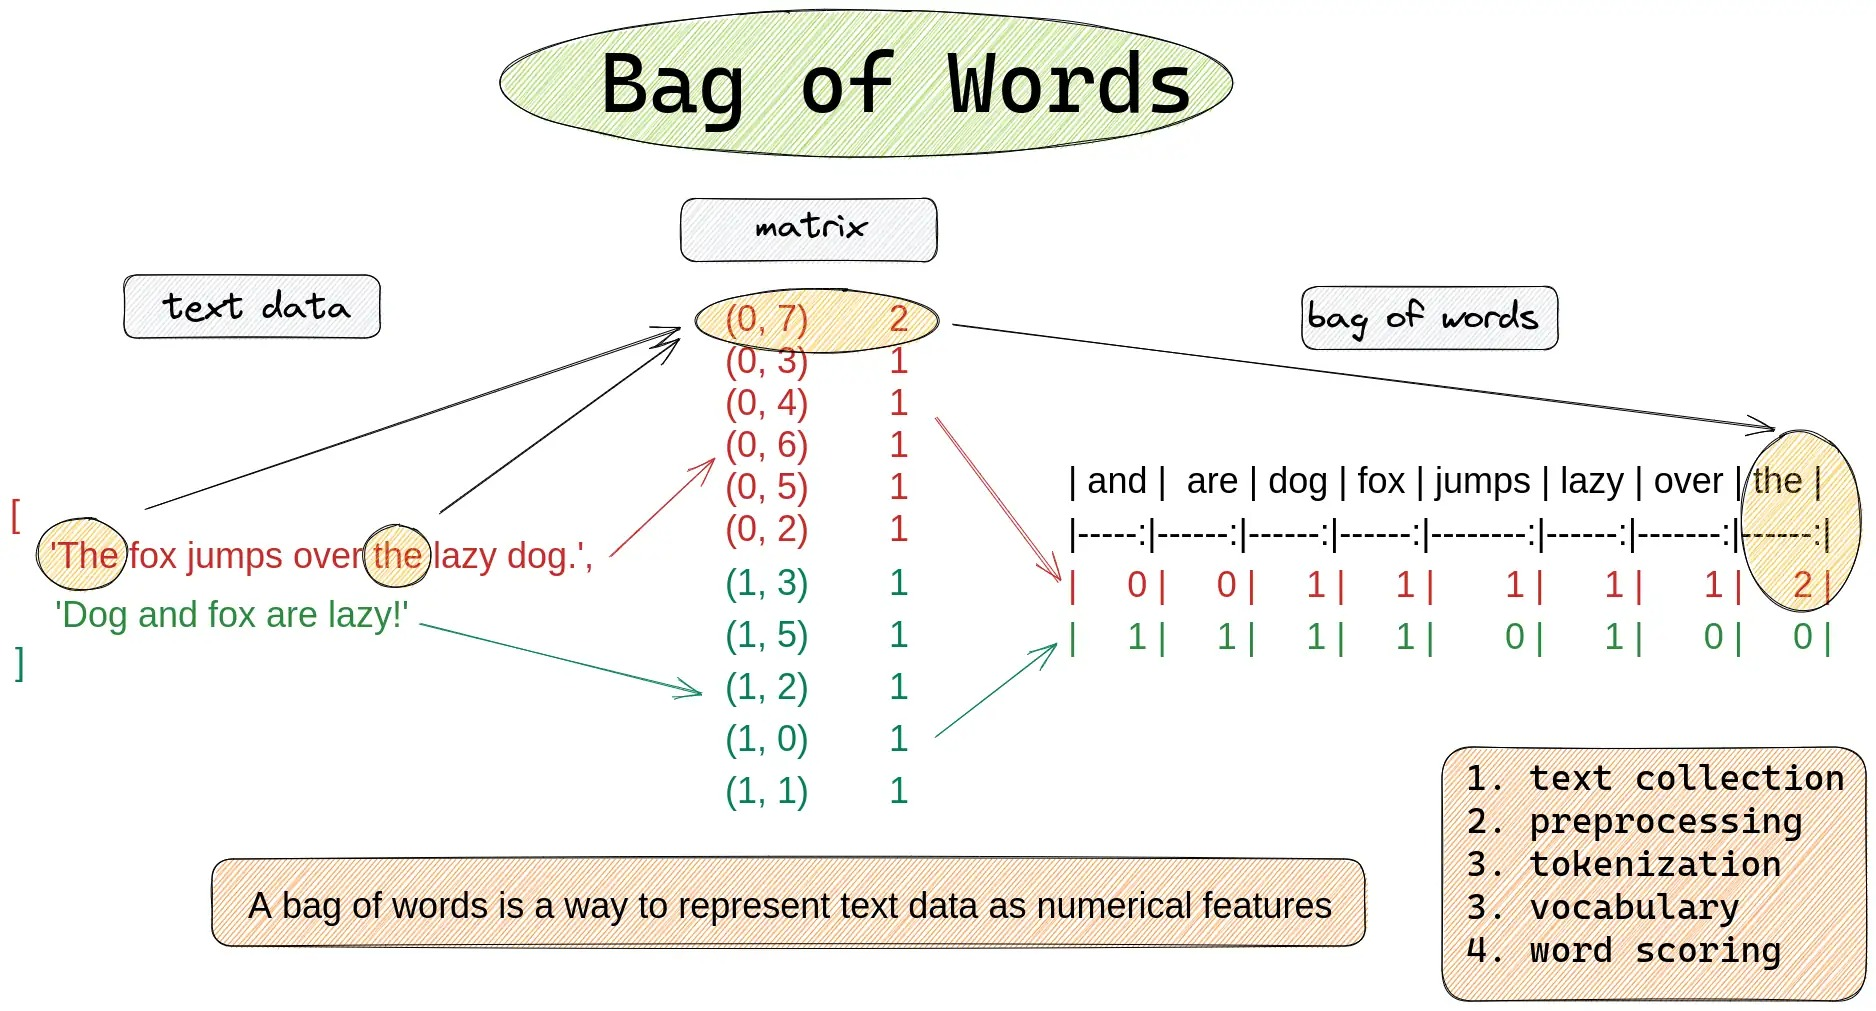
\includegraphics[width=0.84\linewidth]{img/04-bow.jpg}
    \caption{Minh họa mô hình Bag-of-Words}
\end{figure}
\newpage
\section{Phân loại thư rác trên tập dữ liệu Enron-Spam}

\subsection{Tổng quan}
\paragraph{}{Bộ dữ liệu \textbf{Enron-Spam} là một nguồn tài liệu tuyệt vời được thu thập bởi V. Metsis, I. Androutsopoulos và G. Paliouras và được mô tả trong ấn phẩm của họ "Spam Filtering with Naive Bayes - Which Naive Bayes?" \cite{metsis2006spam}. Bộ dữ liệu chứa tổng cộng 17.171 thư rác và
16.545 thư không phải thư rác ("ham") (tổng cộng 33.716 thư điện tử).}

\paragraph{}{Dựa trên kiến thức lý thuyết về Maximum Likelihood Estimation (MLE), Maximum A Posteriori Estimation (MAP) và mô hình Bag-of-Words, chúng tôi sẽ sử dụng mô hình thống kê \textbf{Naive Bayes Classifier} để \textbf{phân loại thư rác} trên bộ dữ liệu Enron-Spam. Quy trình các bước như sau:}

\begin{enumerate}
    \item \textbf{Tải, khám phá và tiền xử lý dữ liệu.}
    \item \textbf{Vector hóa văn bản dựa trên mô hình Bag-of-Words.}
    \item \textbf{Phân loại thư rác bằng Multinomial Naive Bayes.}
    \item \textbf{Đánh giá mô hình bằng độ chính xác, ma trận nhầm lẫn.}
\end{enumerate}

\subsection{Bộ dữ liệu Enron-Spam và tiền xử lý dữ liệu}
\paragraph{}{Bộ dữ liệu \textbf{Enron-Spam} được cung cấp dưới dạng 2 file: \texttt{train.csv} và \texttt{val.csv},  ứng với 2 tập \textbf{training} và \textbf{validation}. Trong đó gồm: 
\begin{itemize}
    \item \texttt{train.csv}: 27284 dòng; 4 cột: \texttt{Message ID}, \texttt{Subject}, \texttt{Message}, \texttt{Spam/Ham}.
    \item \texttt{val.csv}: 3084 dòng; 4 cột: \texttt{Message ID}, \texttt{Subject}, \texttt{Message}, \texttt{Spam/Ham}.
    \begin{itemize}
        \item \texttt{Message ID}: Chỉ số của thư.
        \item \texttt{Subject}: Tiêu đề thư
        \item \texttt{Message}: Nội dung thư.
        \item \texttt{Spam/Ham}: Biến phân loại thư. \texttt{Ham} là thư bình thường, \texttt{Spam} là thư rác.
    \end{itemize}
\end{itemize}

Đây lần lượt là 5 dòng đầu tiên của tập training (\texttt{train.csv}) và tập validation (\texttt{val.csv}):

\begin{figure}[H]
    \centering
    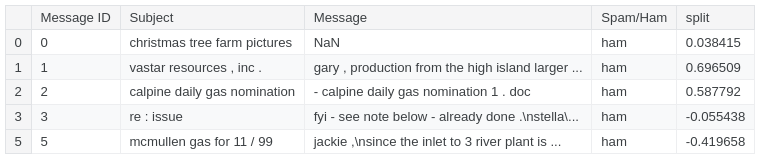
\includegraphics[width=1\linewidth]{img/05-dftrain-head.png}
    \caption{5 dòng đầu tiên của tập train}
\end{figure}

\begin{figure}[H]
    \centering
    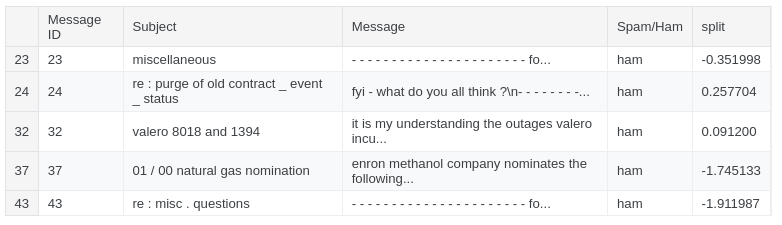
\includegraphics[width=1\linewidth]{img/05-dfval-head.png}
    \caption{5 dòng đầu tiên của tập validation}
\end{figure}

\paragraph{}{Với các bước tiền xử lý dữ liệu, chúng tôi lần lượt áp dụng các kĩ thuật sau:}

\begin{enumerate}
    \item \textbf{Thay thế các ô NaN} (Not-a-Number) bằng chuỗi kí tự rỗng. Chuyển các kí tự chữ thành chữ thường.
    \item \textbf{Gộp chuỗi kí tự} trong hai cột \texttt{Subject} và \texttt{Message} thành một chuỗi kí tự duy nhất và tạo cột mới: \texttt{full\_text}.
    \item \textbf{Chuyển đổi nhãn} của cột \texttt{ham/spam} thành số: \texttt{ham -> 0}, \texttt{spam -> 1}.
\end{enumerate}

\subsection{Vector hóa văn bản bằng Bag-of-Words}

\paragraph{}{Chúng tôi áp dụng phương pháp Bag-of-Words được nhắc đến trong phần \ref{bow-section} để chuyển đổi các chuỗi kí tự trong cột \texttt{full\_text} (được hợp bởi \texttt{Subject} và \texttt{Message}) thành vector. Các vector này có đặc điểm:}

\begin{itemize}
    \item Mỗi vector ứng với một \texttt{full\_text} của một thư. Các vector này biểu diễn tần suất xuất hiện của các từ có trong \texttt{full\_text}.
    \item Kích thước các vector là bằng nhau và bằng với số lượng từ của từ điển được xây dựng trên toàn bộ cột \texttt{full\_text}, theo phương pháp Bag-of-Words.
    \item Mỗi vector có kích thước là \texttt{(1, 37830)}, ứng với số lượng từ có trong từ điển là 37830.
\end{itemize}

\subsection{Multinomial Naive Bayes}
\paragraph{}{Mô hình được sử dụng trong quá trình huấn luyện là \textbf{Multinomial Naive Bayes}, một mô hình xác suất dựa trên \textit{định lý Bayes} với giả định ``naive'' rằng các đặc trưng là \textit{độc lập có điều kiện} khi biết nhãn lớp. Đây là lựa chọn đặc biệt phù hợp trong các bài toán phân loại văn bản, nơi mà đặc trưng của dữ liệu là \textit{tần suất xuất hiện của từ} trong tài liệu.}

\subsubsection{Huấn luyện mô hình (fit)}

\textbf{Mục tiêu:} Học các tham số của mô hình từ tập dữ liệu huấn luyện.

\textbf{Quy trình huấn luyện:}
\begin{enumerate}
    \item \textbf{Xây dựng từ điển}: Thu thập tất cả các từ xuất hiện trong tập dữ liệu huấn luyện để tạo không gian đặc trưng.
    \item \textbf{Vector hóa dữ liệu}: Biểu diễn các văn bản dưới dạng ma trận BoW (\textit{Bag-of-Words}).
    \item \textbf{Tính log xác suất tiên nghiệm $P(c)$}:
    \[
    P(c) = \frac{N_c}{N}
    \]
    trong đó $N_c$ là số lượng mẫu thuộc lớp $c$, và $N$ là tổng số mẫu trong tập huấn luyện.
    \item \textbf{Tính tổng số từ xuất hiện trong mỗi lớp}.
    \item \textbf{Tính log xác suất có điều kiện (likelihood)} $P(\text{word}_i \mid c)$ cho mỗi từ và mỗi lớp.
\end{enumerate}

\subsubsection{Dự đoán log xác suất hậu nghiệm cho một vector BoW thưa}

\textbf{Mục tiêu:} Tính toán \textit{log của tử số xác suất hậu nghiệm} cho một văn bản (biểu diễn dưới dạng vector BoW thưa) tương ứng với từng lớp.

Với mỗi văn bản $x^{(i)}$, mô hình tính:
\[
\log P(c) + \sum_{j} x^{(i)}_j \cdot \log P(\text{word}_j \mid c)
\]
trong đó $x^{(i)}_j$ là số lần từ thứ $j$ xuất hiện trong văn bản $x^{(i)}$.

Không áp dụng phép chuẩn hoá (tức không chia cho mẫu số), vì ta chỉ cần so sánh tương đối giữa các lớp.

Nhãn dự đoán $\hat{y}^{(i)}$ được xác định theo nguyên lý \textbf{Maximum A Posteriori (MAP)}:
\[
\hat{y}^{(i)} = \arg\max_{c \in \mathcal{C}} \left( \log P(c) + \sum_{j} x^{(i)}_j \cdot \log P(\text{word}_j \mid c) \right)
\]

Quá trình này được áp dụng cho mọi $i = 1, \ldots, n$, tạo thành vector dự đoán:
\[
\hat{y} = [\hat{y}^{(1)}, \hat{y}^{(2)}, \ldots, \hat{y}^{(n)}]
\]

\subsection{Đánh giá mô hình}

\paragraph{}{Ở bước đánh giá mô hình, chúng tôi sử dụng 2 phương pháp chính là \textbf{độ chính xác} (accuracy) và \textbf{ma trận nhầm lẫn} (confusion matrix).}
\begin{itemize}
    \item \textbf{Độ chính xác:} Được tính bằng số trường hợp mô hình phân loại \texttt{ham/spam} đúng trên tổng số trường hợp cần phân loại.
    \item \textbf{Ma trận nhầm lẫn}: Phương pháp đánh giá hiệu suất của bài toán phân loại, trong đó:
    \begin{itemize}
        \item TP (True Positive): Số lượng thư \texttt{spam} được phân loại đúng. 
        \item TN (True Negative): Số lượng thư \texttt{ham} được phân loại đúng. 
        \item FP (False Positive - Type 1 Error): Số lượng thư \texttt{ham} bị phân loại sai thành \texttt{spam}. 
        \item FN (False Negative - Type 2 Error): Số lượng thư \texttt{spam} bị phân loại sai thành \texttt{ham}. 
    \end{itemize}
\end{itemize}

\begin{figure}[H] 
    \centering 

    \begin{subfigure}[b]{0.48\textwidth} 
        \centering
        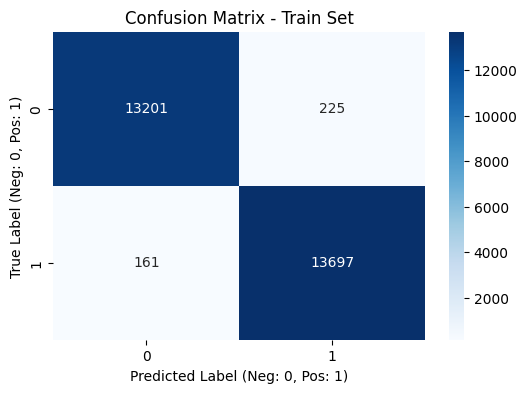
\includegraphics[width=\linewidth]{img/confusion_matrix_train_set.png}
        \caption{Độ chính xác trên tập Training: 0.9893}
        \label{fig:training_results}
    \end{subfigure}
    \hfill 
    \begin{subfigure}[b]{0.48\textwidth} 
        \centering
        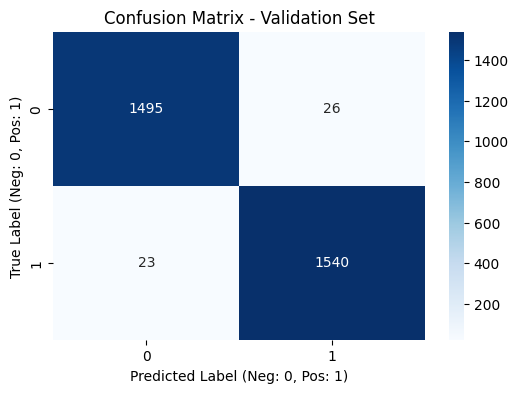
\includegraphics[width=\linewidth]{img/confusion_matrix_valid_set.png}
        \caption{Độ chính xác trên tập Validation: 0.9857}
        \label{fig:validation_results}
    \end{subfigure}

    \caption{Ma trận nhầm lẫn của mô hình trên tập training và validation} 
    \label{fig:overall_results}
\end{figure}
% \newpage
\section{Đánh giá, kết luận}

\paragraph{}{Qua quá trình thực hiện báo cáo \textit{Lab 3 - Phân loại thư rác}, nhóm đã thành công trong việc tìm hiểu và tự lập trình xây dựng một mô hình \textit{Naive Bayes Classifier}. Mô hình được xây dựng dựa trên các kiến thức nền tảng về lý thuyết xác suất, \textit{Định lý Bayes}, cùng với các kỹ thuật ước lượng tham số như \textit{Maximum Likelihood Estimation (MLE)} cho xác suất tiên nghiệm của lớp và \textit{Maximum A Posteriori (MAP) Estimation} (thông qua \textit{Laplace Smoothing}) cho xác suất có điều kiện của từ. Nguyên tắc \textit{Bag-of-Words} đã được áp dụng hiệu quả để biểu diễn dữ liệu văn bản, tập trung vào tần suất xuất hiện của từ mà bỏ qua cấu trúc ngữ pháp phức tạp.}

\paragraph{}{Khi được huấn luyện và đánh giá trên bộ dữ liệu \textit{Enron-Spam}, mô hình của nhóm đã đạt được độ chính xác tổng thể trên 98.9\% trên tập huấn luyện và 98.5\% trên tập kiểm định, cho thấy khả năng học tốt các đặc điểm của dữ liệu và khả năng tổng quát hóa cao trên dữ liệu mới chưa từng thấy. Các chỉ số đánh giá chi tiết như Precision, Recall, và F1-Score cho cả hai lớp \texttt{``ham''} và \texttt{``spam''} đều ở mức rất cao (trên 0.98), phản ánh sự cân bằng và hiệu quả của mô hình trong việc vừa phát hiện chính xác thư rác, vừa hạn chế tối đa việc phân loại nhầm thư hợp lệ. Ma trận nhầm lẫn cũng cho thấy số lượng False Positives (23 trên tập validation) và False Negatives (26 trên tập validation) là tương đối thấp, khẳng định tính thực tiễn của giải pháp.}

\paragraph{}{Việc tự lập trình mô hình \textit{Naive Bayes Classifier} đã giúp nhóm hiểu sâu hơn và có thể áp dụng thực tiễn kiến thức nền tảng về lý thuyết xác suất, cùng các kỹ thuật MLE, MAP được học ở trên lớp để đảm bảo xây dựng mô hình hoạt động ổn định và hiệu quả.}

\newpage
\bibliographystyle{unsrt}
\bibliography{ref/ref}

% \appendix
% \section{Phụ lục}
\begin{itemize}
\item Template này \textbf{không phải} là template chính thức của Khoa Công nghệ thông tin - Trường Đại học Khoa học Tự nhiên.
\item Các hình ảnh, bảng biểu, thuật toán trong template chỉ mang tính chất ví dụ.
\item Nhóm tác giả phân phối \textbf{miễn phí} template này \href{https://github.com/khongsomeo/hcmus-unofficial-report-template}{trên GitHub} và \href{https://www.overleaf.com/latex/templates/hcmus-report-template/zyrhmsxynwqs}{trên Overleaf} với \href{https://github.com/khongsomeo/hcmus-unofficial-report-template/blob/main/LICENSE}{Giấy phép GNU General Public License v3.0}. Nhóm tác giả không chịu trách nhiệm với các bản phân phối không nằm trong hai kênh phân phối chính thức nêu trên.
\end{itemize}


\end{document}